% Options for packages loaded elsewhere
% Options for packages loaded elsewhere
\PassOptionsToPackage{unicode}{hyperref}
\PassOptionsToPackage{hyphens}{url}
\PassOptionsToPackage{dvipsnames,svgnames,x11names}{xcolor}
%
\documentclass[
  11pt,
  a4paper,
]{article}
\usepackage{xcolor}
\usepackage[margin=2.2cm]{geometry}
\usepackage{amsmath,amssymb}
\setcounter{secnumdepth}{5}
\usepackage{iftex}
\ifPDFTeX
  \usepackage[T1]{fontenc}
  \usepackage[utf8]{inputenc}
  \usepackage{textcomp} % provide euro and other symbols
\else % if luatex or xetex
  \usepackage{unicode-math} % this also loads fontspec
  \defaultfontfeatures{Scale=MatchLowercase}
  \defaultfontfeatures[\rmfamily]{Ligatures=TeX,Scale=1}
\fi
\usepackage{lmodern}
\ifPDFTeX\else
  % xetex/luatex font selection
\fi
% Use upquote if available, for straight quotes in verbatim environments
\IfFileExists{upquote.sty}{\usepackage{upquote}}{}
\IfFileExists{microtype.sty}{% use microtype if available
  \usepackage[]{microtype}
  \UseMicrotypeSet[protrusion]{basicmath} % disable protrusion for tt fonts
}{}
\makeatletter
\@ifundefined{KOMAClassName}{% if non-KOMA class
  \IfFileExists{parskip.sty}{%
    \usepackage{parskip}
  }{% else
    \setlength{\parindent}{0pt}
    \setlength{\parskip}{6pt plus 2pt minus 1pt}}
}{% if KOMA class
  \KOMAoptions{parskip=half}}
\makeatother
% Make \paragraph and \subparagraph free-standing
\makeatletter
\ifx\paragraph\undefined\else
  \let\oldparagraph\paragraph
  \renewcommand{\paragraph}{
    \@ifstar
      \xxxParagraphStar
      \xxxParagraphNoStar
  }
  \newcommand{\xxxParagraphStar}[1]{\oldparagraph*{#1}\mbox{}}
  \newcommand{\xxxParagraphNoStar}[1]{\oldparagraph{#1}\mbox{}}
\fi
\ifx\subparagraph\undefined\else
  \let\oldsubparagraph\subparagraph
  \renewcommand{\subparagraph}{
    \@ifstar
      \xxxSubParagraphStar
      \xxxSubParagraphNoStar
  }
  \newcommand{\xxxSubParagraphStar}[1]{\oldsubparagraph*{#1}\mbox{}}
  \newcommand{\xxxSubParagraphNoStar}[1]{\oldsubparagraph{#1}\mbox{}}
\fi
\makeatother


\usepackage{longtable,booktabs,array}
\usepackage{calc} % for calculating minipage widths
% Correct order of tables after \paragraph or \subparagraph
\usepackage{etoolbox}
\makeatletter
\patchcmd\longtable{\par}{\if@noskipsec\mbox{}\fi\par}{}{}
\makeatother
% Allow footnotes in longtable head/foot
\IfFileExists{footnotehyper.sty}{\usepackage{footnotehyper}}{\usepackage{footnote}}
\makesavenoteenv{longtable}
\usepackage{graphicx}
\makeatletter
\newsavebox\pandoc@box
\newcommand*\pandocbounded[1]{% scales image to fit in text height/width
  \sbox\pandoc@box{#1}%
  \Gscale@div\@tempa{\textheight}{\dimexpr\ht\pandoc@box+\dp\pandoc@box\relax}%
  \Gscale@div\@tempb{\linewidth}{\wd\pandoc@box}%
  \ifdim\@tempb\p@<\@tempa\p@\let\@tempa\@tempb\fi% select the smaller of both
  \ifdim\@tempa\p@<\p@\scalebox{\@tempa}{\usebox\pandoc@box}%
  \else\usebox{\pandoc@box}%
  \fi%
}
% Set default figure placement to htbp
\def\fps@figure{htbp}
\makeatother





\setlength{\emergencystretch}{3em} % prevent overfull lines

\providecommand{\tightlist}{%
  \setlength{\itemsep}{0pt}\setlength{\parskip}{0pt}}



 


\usepackage{booktabs}
\usepackage{longtable}
\usepackage{array}
\usepackage{multirow}
\usepackage{wrapfig}
\usepackage{float}
\usepackage{colortbl}
\usepackage{pdflscape}
\usepackage{tabu}
\usepackage{threeparttable}
\usepackage{threeparttablex}
\usepackage[normalem]{ulem}
\usepackage{makecell}
\usepackage{xcolor}
\usepackage{fancyhdr}
\usepackage{setspace}
\usepackage{tocloft}
\pagestyle{fancy}
\fancyhf{}
\rhead{\thepage}
\renewcommand{\headrulewidth}{0pt}
\makeatletter
\@ifpackageloaded{caption}{}{\usepackage{caption}}
\AtBeginDocument{%
\ifdefined\contentsname
  \renewcommand*\contentsname{Table of contents}
\else
  \newcommand\contentsname{Table of contents}
\fi
\ifdefined\listfigurename
  \renewcommand*\listfigurename{List of Figures}
\else
  \newcommand\listfigurename{List of Figures}
\fi
\ifdefined\listtablename
  \renewcommand*\listtablename{List of Tables}
\else
  \newcommand\listtablename{List of Tables}
\fi
\ifdefined\figurename
  \renewcommand*\figurename{Figure}
\else
  \newcommand\figurename{Figure}
\fi
\ifdefined\tablename
  \renewcommand*\tablename{Table}
\else
  \newcommand\tablename{Table}
\fi
}
\@ifpackageloaded{float}{}{\usepackage{float}}
\floatstyle{ruled}
\@ifundefined{c@chapter}{\newfloat{codelisting}{h}{lop}}{\newfloat{codelisting}{h}{lop}[chapter]}
\floatname{codelisting}{Listing}
\newcommand*\listoflistings{\listof{codelisting}{List of Listings}}
\makeatother
\makeatletter
\makeatother
\makeatletter
\@ifpackageloaded{caption}{}{\usepackage{caption}}
\@ifpackageloaded{subcaption}{}{\usepackage{subcaption}}
\makeatother
\usepackage{bookmark}
\IfFileExists{xurl.sty}{\usepackage{xurl}}{} % add URL line breaks if available
\urlstyle{same}
\hypersetup{
  colorlinks=true,
  linkcolor={blue},
  filecolor={Maroon},
  citecolor={Blue},
  urlcolor={Blue},
  pdfcreator={LaTeX via pandoc}}


\author{}
\date{}
\begin{document}


\thispagestyle{empty}

\vspace*{3cm}

\begin{center}
{\Large \textbf{Housing Lending, Overseas Migration and Wage Growth Across Australian States}}\\[0.8cm]

{\large Data Exploration Project}\\[1.8cm]

TingTing Wu\\
Student ID: 35717343\\[1.2cm]

FIT5147 Data Exploration and Visualization\\
Semester 1, 2026\\
Monash University\\[1.2cm]

29 March 2026
\end{center}

\newpage

\thispagestyle{plain}
\begin{center}
\section*{Contents}
\end{center}

\tableofcontents

\newpage

\section{Introduction}\label{introduction}

This report, \emph{Housing Lending, Overseas Migration and Wage Growth
Across Australian States}, examines housing affordability in Australia,
a major social and economic issue. Public debate often links housing
pressure to migration, limited supply, and weak wage growth. For
example, SBS News (2026) discussed whether high migration is truly
supported by evidence as a cause of the housing crisis. This makes the
topic important for households, workers, students, and policy makers.

The report explores how housing lending, overseas migration, and wage
growth have changed across Australian states over time. Using Australian
Bureau of Statistics data, it examines owner-occupier lending, investor
lending, net overseas migration, and the Wage Price Index. The aim is to
assess whether common public claims about migration, wages, and housing
stress are reflected in the data, and whether these patterns differ by
state.

I am personally interested in this topic because, as an international
student from Taiwan living in Melbourne, I have become more aware of
housing affordability pressures. Seeing how difficult high housing costs
can make financial security for students and workers motivated me to
examine this issue using data rather than relying only on public opinion
or media debate.

This report addresses the following questions:

\begin{enumerate}
\def\labelenumi{\arabic{enumi}.}
\tightlist
\item
  Does the growth of housing lending align with wage growth across
  Australian states, and how has the lending structure changed over
  time?
\item
  How have the origins of overseas migrants and their state settlement
  patterns changed across Australian states over time?
\item
  Where are the largest gaps between investor lending and migration
  demand across Australian states, and how have these gaps changed over
  time?
\end{enumerate}

\section{Data Wrangling and Checking}\label{data-wrangling-and-checking}

This project uses four open datasets from the Australian Bureau of
Statistics (ABS): Net Overseas Migration by Country of Birth,
Owner-Occupier Lending, Investor Lending, and the Wage Price Index. The
direct download links are provided below:

\begin{itemize}
\tightlist
\item
  \href{https://www.abs.gov.au/statistics/people/population/overseas-migration/latest-release/34070DO001_202425.xlsx}{Net
  Overseas Migration by Country of Birth}
\item
  \href{https://www.abs.gov.au/statistics/economy/finance/lending-indicators/latest-release/560104.xlsx}{Owner-Occupier
  Lending}
\item
  \href{https://www.abs.gov.au/statistics/economy/finance/lending-indicators/latest-release/560114.xlsx}{Investor
  Lending}
\item
  \href{https://www.abs.gov.au/statistics/economy/price-indexes-and-inflation/wage-price-index-australia/latest-release/634502b.xlsx}{Wage
  Price Index}
\end{itemize}

Before checking and cleaning the data, I first transformed the three ABS
datasets into tidy formats that were easier to compare and analyse in R.
Although all three sources were downloaded as Excel workbooks, they had
different internal structures and could not be used directly for
analysis.

For the overseas migration data, the workbook contained nine separate
tables, including one national table and eight state or territory
tables. I created a lookup table containing the sheet names, state
names, and row ranges, then used a function to read each worksheet in
the same way. In each sheet, I used the first imported row as the column
names, renamed the first two columns as \texttt{sacc\_code} and
\texttt{country\_of\_birth}, and removed note labels from the year
columns, which is the letter attached to 2024-25. I then converted the
data from wide format to long format using \texttt{pivot\_longer()}, so
that each row represented one state, one country of birth, and one
financial year. Finally, I combined all nine sheets into a single
dataset called \texttt{overseas\_migration}.

For the housing finance data, I used the \texttt{Data1} sheet from both
the owner-occupier and investor lending workbooks. In both files, the
first ten rows contained metadata rather than observations, so I read
these rows separately from the main time series data. I created
temporary column names for the series columns and extracted key metadata
such as state, value type, unit, and series type by splitting the
original ABS series description. I then reshaped the time series data
into long format and created additional time variables, including
calendar year, quarter, and financial year. After that, I combined the
owner-occupier and investor datasets into one dataset called
\texttt{housing\_finance}, with an added variable called
\texttt{loan\_type} to distinguish between the two sources.

For the Wage Price Index data, I again used the \texttt{Data1} sheet and
followed a similar process. I read the metadata rows separately, created
temporary series column names, and extracted information such as state,
wage measure, and unit from the ABS series descriptions. I then reshaped
the data into long format and created year, quarter, and financial year
variables. This produced a final tidy dataset called
\texttt{wage\_price\_index}.

Overall, the main purpose of this step was to convert the original Excel
workbooks into consistent long-format datasets that could be compared
more easily across states and time. This also made it easier to carry
out the next stage of the project, which involved checking the
structure, identifying missing values, reviewing inconsistencies, and
cleaning the data where necessary. The tidy datasets and all data
processing code used in this project are available in my
\href{https://github.com/ruby910113/FIT5147-DEP-report}{GitHub
repository}.

\subsection{Creating a Common Financial Year
Structure}\label{creating-a-common-financial-year-structure}

As shown in Table~\ref{tbl-time-summary}, Housing finance and Wage price
index are quarterly datasets recorded using calendar year and month,
while Overseas migration is recorded by financial year. To make the
three datasets easier to compare, I created a financial year variable
for the quarterly datasets based on the quarter-ending months of
September, December, March, and June. The datasets also have different
time ranges, since Housing finance and Wage price index start earlier
than Overseas migration. Therefore, I restricted all three datasets to
the shared financial-year period from 2004-05 to 2024-25 before carrying
out the analysis.

\begin{longtable}[t]{lllll}

\caption{\label{tbl-time-summary}Summary of time structure across the
datasets}

\tabularnewline

\\
\toprule
Dataset & Start (Year/Month) & End (Year/Month) & Frequency & Time period\\
\midrule
Overseas migration & Not applicable & Not applicable & Annual & 2004-05 to 2024-25\\
Housing finance & 2002/9 & 2025/12 & Quarterly & 2002-03 to 2025-26\\
Wage price index & 1997/9 & 2025/12 & Quarterly & 1997-98 to 2025-26\\
\bottomrule

\end{longtable}

\subsection{Understanding Missing Values in the Housing Finance
Data}\label{understanding-missing-values-in-the-housing-finance-data}

Table~\ref{tbl-hf-missing-summary} shows that the housing finance
dataset is largely complete, except for the Investor Number series,
which is only available from 2019-20 onward. This suggests that the
missing values are structural rather than accidental, since the series
begins later in the original source data. Therefore, these values were
not imputed, and any analysis using Investor Number should be limited to
2019-20 onward or interpreted cautiously when compared with the longer
series.

\begin{longtable}[t]{llllrr}

\caption{\label{tbl-hf-missing-summary}Series start and end dates in the
original housing finance workbooks}

\tabularnewline

\\
\toprule
Loan type & Value type & First FY & Last FY & Missing values & Available values\\
\midrule
Investor & Number & 2019-20 & 2024-25 & 1620 & 648\\
Investor & Value & 2004-05 & 2024-25 & 0 & 2268\\
Owner-occupier & Number & 2004-05 & 2024-25 & 0 & 2268\\
Owner-occupier & Value & 2004-05 & 2024-25 & 0 & 2268\\
\bottomrule

\end{longtable}

\subsection{Checking Distribution Shapes Across the
Datasets}\label{checking-distribution-shapes-across-the-datasets}

Figure~\ref{fig-distribution} shows no clear sign of major data errors
after the asinh transformation. The housing finance data are
right-skewed, but the distribution is still fairly smooth, so this looks
more like normal variation than unusual mistakes. The overseas migration
data are strongly concentrated around zero, with longer tails on both
sides, which suggests that many observations are small or zero while
some are much larger in either the positive or negative direction. The
wage price index data show a clear bimodal shape, but this is likely due
to combining index values and percentage change measures in the same
dataset, rather than indicating abnormal observations. Overall, this
check suggests that the main issue is differences in data structure
across the datasets, not obvious errors in the values.

\begin{figure}

\centering{

\pandocbounded{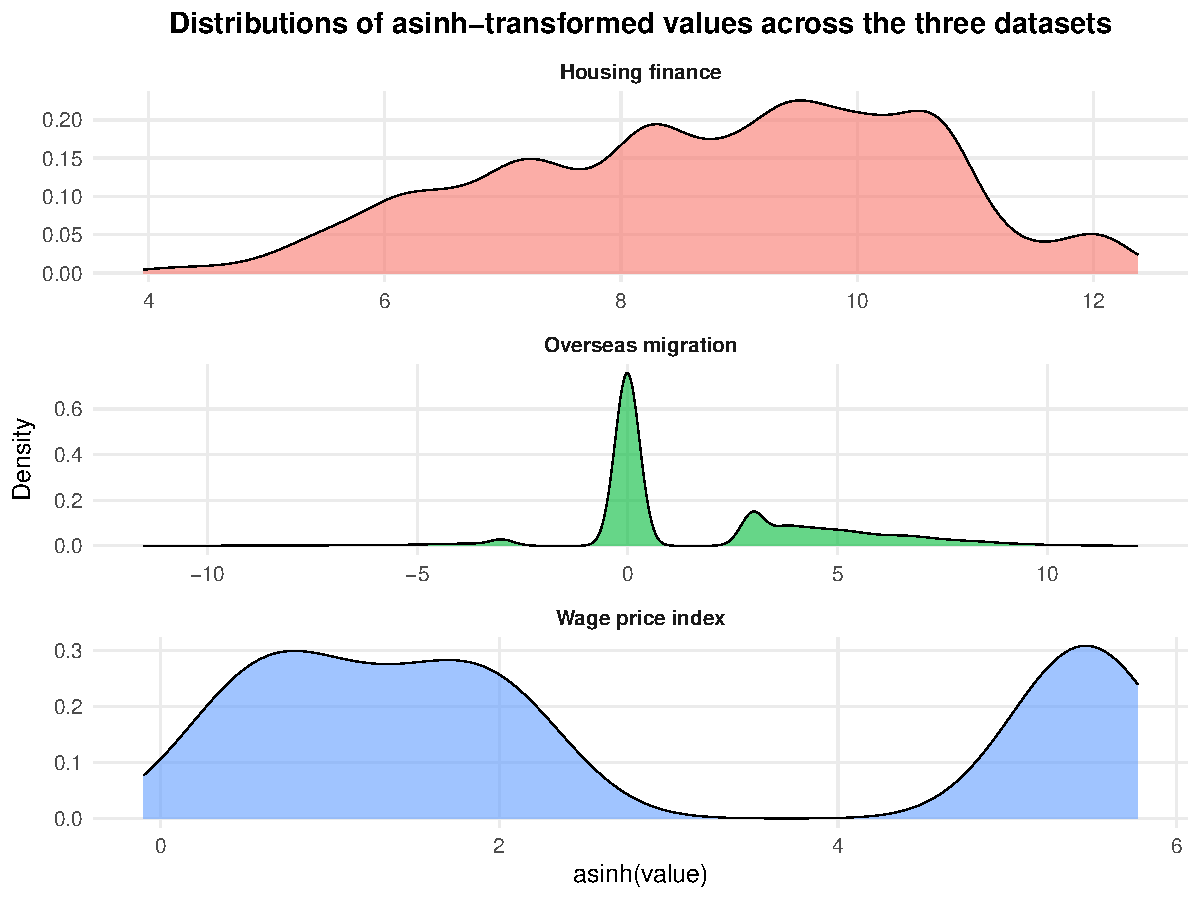
\includegraphics[keepaspectratio]{DEP_Wu_35717343_files/figure-pdf/fig-distribution-1.pdf}}

}

\caption{\label{fig-distribution}}

\end{figure}%

\subsection{Summary of Data Checking}\label{summary-of-data-checking}

Overall, the data wrangling and checking steps suggest that the three
datasets were successfully converted into tidy formats and aligned to a
common financial-year structure for comparison. No major data quality
problems were identified, aside from the structurally missing Investor
Number series and the expected differences in measurement scales across
the datasets. These issues were taken into account in later analysis, so
the cleaned data provide a suitable basis for exploring relationships
between migration, housing lending, and wage growth across Australian
states.

\section{Data Exploration}\label{data-exploration}

This section explores the \textbf{relationships between housing lending,
overseas migration, and wage growth across Australian states} using
financial-year summaries and composition measures from \textbf{2004-05
to 2024-25}.

\subsection{Housing Lending, Wage Growth and Lending Structure Across
Australian
States}\label{housing-lending-wage-growth-and-lending-structure-across-australian-states}

To address the first research question, I compared annual housing
lending growth with annual wage growth across Australian states from
2005-06 to 2024-25. I then examined whether these two measures moved
together over time, and how the investor share of total lending value
changed across states.

\subsubsection{Divergence between housing lending growth and wage
growth}\label{divergence-between-housing-lending-growth-and-wage-growth}

Figure~\ref{fig-q1-overall-growth} separates housing lending growth and
wage growth into two panels, making their state-level patterns easier to
compare. Wage growth stays within a relatively narrow range of about
1.5\% to 4.2\%, but still shows a longer-run decline from 2005-06 to
2020-21 before rising again towards its period average of 3\%. Western
Australia shows the largest swings in wage growth, while Tasmania
appears least affected during the COVID-19 period and rebounds strongly
afterwards.

By contrast, housing lending growth is much more volatile and differs
more across states. The sharp divergence in 2020-21 likely reflects the
COVID-19 period, while the large fall in 2022-23 is consistent with a
post-pandemic adjustment. Lending fluctuations are especially large in
Northern Territory, Western Australia, and New South Wales, whereas
South Australia and the Australian Capital Territory are relatively more
stable. Overall, the figure suggests that short-run changes in housing
finance are driven much more by lending market conditions than by wage
growth.

\begin{figure}

\centering{

\pandocbounded{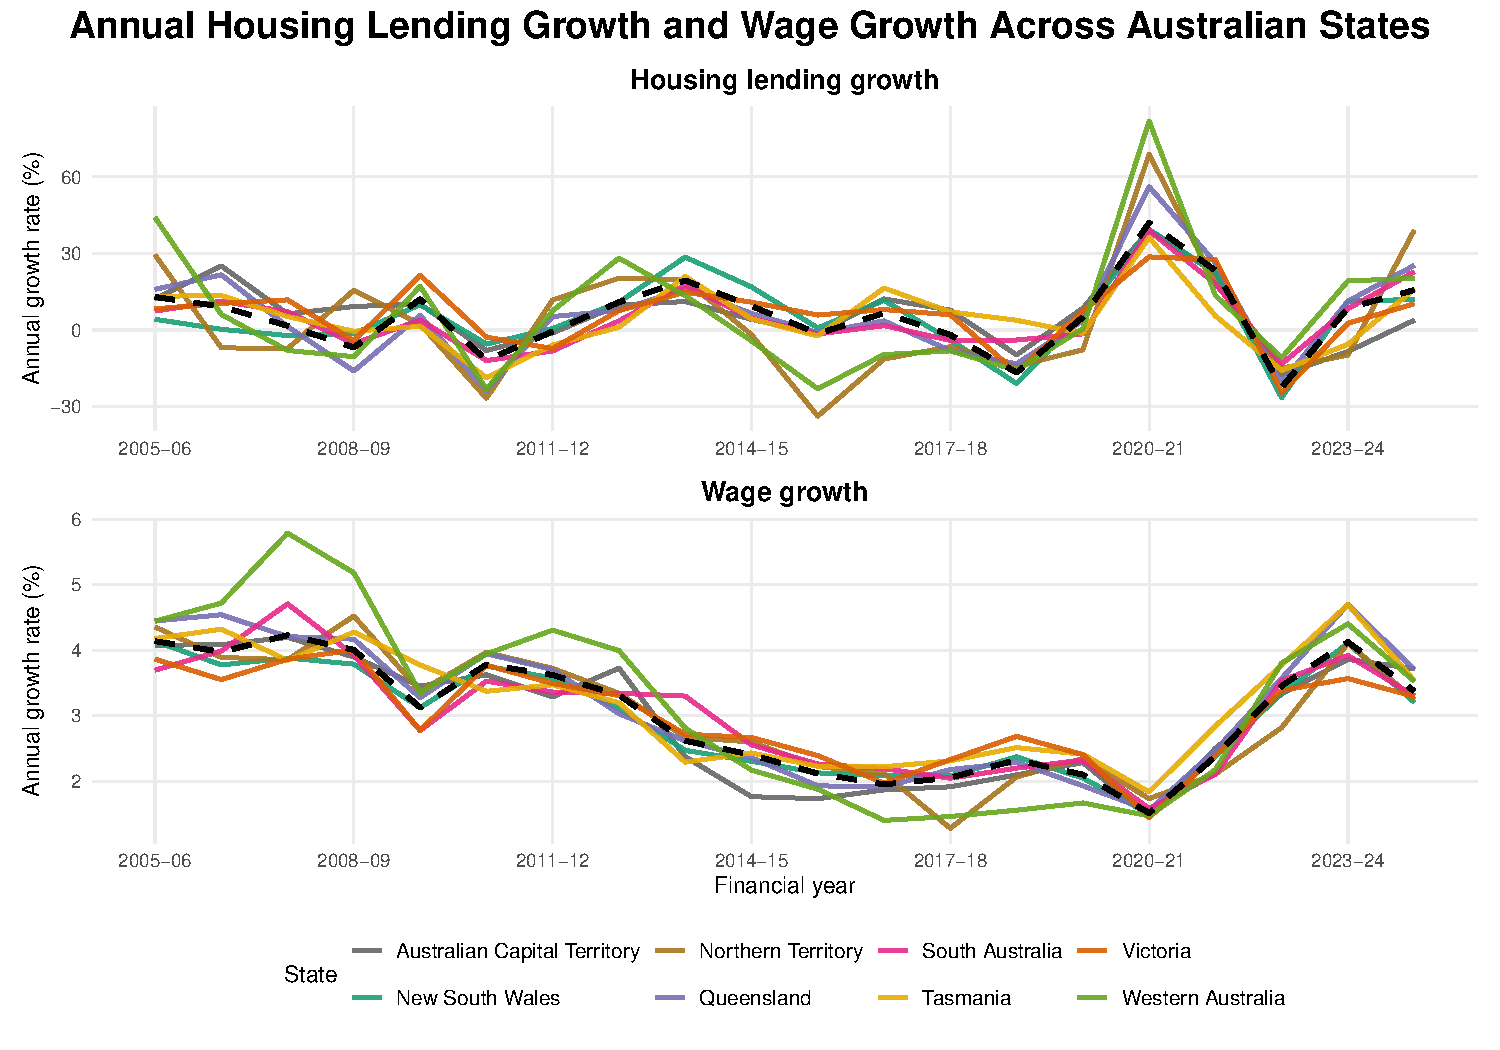
\includegraphics[keepaspectratio]{DEP_Wu_35717343_files/figure-pdf/fig-q1-overall-growth-1.pdf}}

}

\caption{\label{fig-q1-overall-growth}Annual housing lending growth and
wage growth across Australian states, 2005-06 to 2024-25. Coloured lines
show individual states and the dashed black line shows the Total
Australia series.}

\end{figure}%

\subsubsection{Long-run changes in the investor share of lending
value}\label{long-run-changes-in-the-investor-share-of-lending-value}

Figure~\ref{fig-q1-structure-value} examines how the investor share of
total housing lending value changed across states from 2004-05 to
2024-25. The national pattern is clearly cyclical. The investor share
starts at about 38.3\%, rises to a peak of 44.5\% in 2014-15, then falls
sharply to 25.4\% in 2020-21 before recovering to 37.8\% by 2024-25.

New South Wales stands out as the most investor-oriented market over the
long run. Its average investor share is about 39.6\%, and it remains
above the national share in 81\% of years, peaking at 53.9\% in 2014-15.
By contrast, Tasmania has one of the lowest average investor shares, at
about 25.8\%. Northern Territory and Tasmania show a somewhat similar
long-run pattern, with investor shares generally remaining below the
national benchmark for much of the period. However, both rise sharply
after the COVID-19 period. By 2024-25, Northern Territory reaches 40.5\%
and Tasmania reaches 26.2\%, compared with the national share of 37.8\%.
Western Australia follows a different pattern: after 2008-09, its
investor share begins to move further away from the national benchmark,
before recovering again after the 2020-21 low. It rises from 16.1\% in
2020-21 to 36.8\% in 2024-25. The other states generally follow the
national cycle more closely and do not show such distinctive departures.
Overall, the figure suggests that the structure of housing lending has
changed substantially over time and that investor activity has been much
more important in some state housing markets than in others.

\begin{figure}

\centering{

\pandocbounded{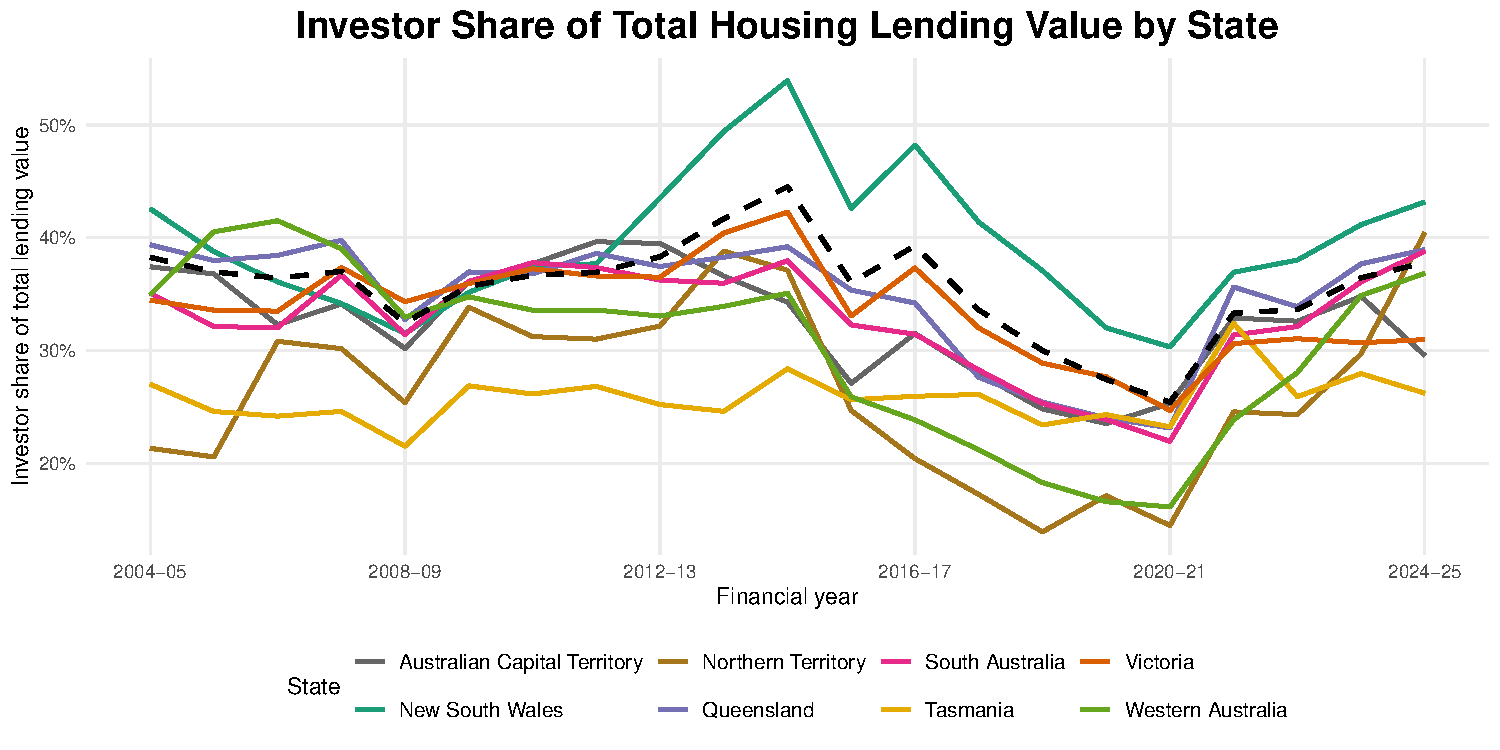
\includegraphics[keepaspectratio]{DEP_Wu_35717343_files/figure-pdf/fig-q1-structure-value-1.pdf}}

}

\caption{\label{fig-q1-structure-value}Investor share of total housing
lending value across Australian states, 2004-05 to 2024-25. Coloured
lines show individual states and the dashed black line shows the Total
Australia share.}

\end{figure}%

\subsubsection{Summary of findings}\label{summary-of-findings}

Overall, Figure~\ref{fig-q1-overall-growth} and
Figure~\ref{fig-q1-structure-value} suggest that housing lending growth
does not closely track wage growth across Australian states, and that
the structure of lending has changed markedly over time. Investor
activity appears to be more strongly related to the composition of
lending than to short-run movements in total lending growth, with some
states remaining much more investor-oriented than others.

\subsection{Changing Migrant Origins, State Settlement Patterns, and
Their Links to Wage Growth and Housing Lending in
Australia}\label{changing-migrant-origins-state-settlement-patterns-and-their-links-to-wage-growth-and-housing-lending-in-australia}

To address the second research question, I examined how the origins of
overseas migrants changed across Australian states from 2004-05 to
2024-25. I then examined whether migrant-origin concentration within
each state was associated with wage growth and housing lending growth.

\subsubsection{Changing Origins of Migrant Inflows Across Australian
States}\label{changing-origins-of-migrant-inflows-across-australian-states}

Figure~\ref{fig-q2-origin-heatmap} shows a clear long-run shift in the
origins of migrant inflows across most states. The most striking pattern
is the rising importance of Southern and Central Asia, whose national
share of positive overseas migrant inflows increases from about 15.6\%
in 2004-05 to 36.3\% in 2024-25. This rise appears across nearly all
states, but is especially strong in the Australian Capital Territory and
Victoria, where Southern and Central Asia accounts for about 55.6\% and
41.0\% of positive inflows respectively in 2024-25.

By contrast, North-West Europe becomes less important in most states,
although it remains more prominent in Western Australia, where it still
accounts for about 21.0\% of positive inflows in 2024-25. Overall,
migrant settlement patterns remain uneven across states, with Victoria
and the Australian Capital Territory becoming more concentrated in
Southern and Central Asian inflows, while Western Australia retains a
more visible North-West European component.

\begin{figure}

\centering{

\pandocbounded{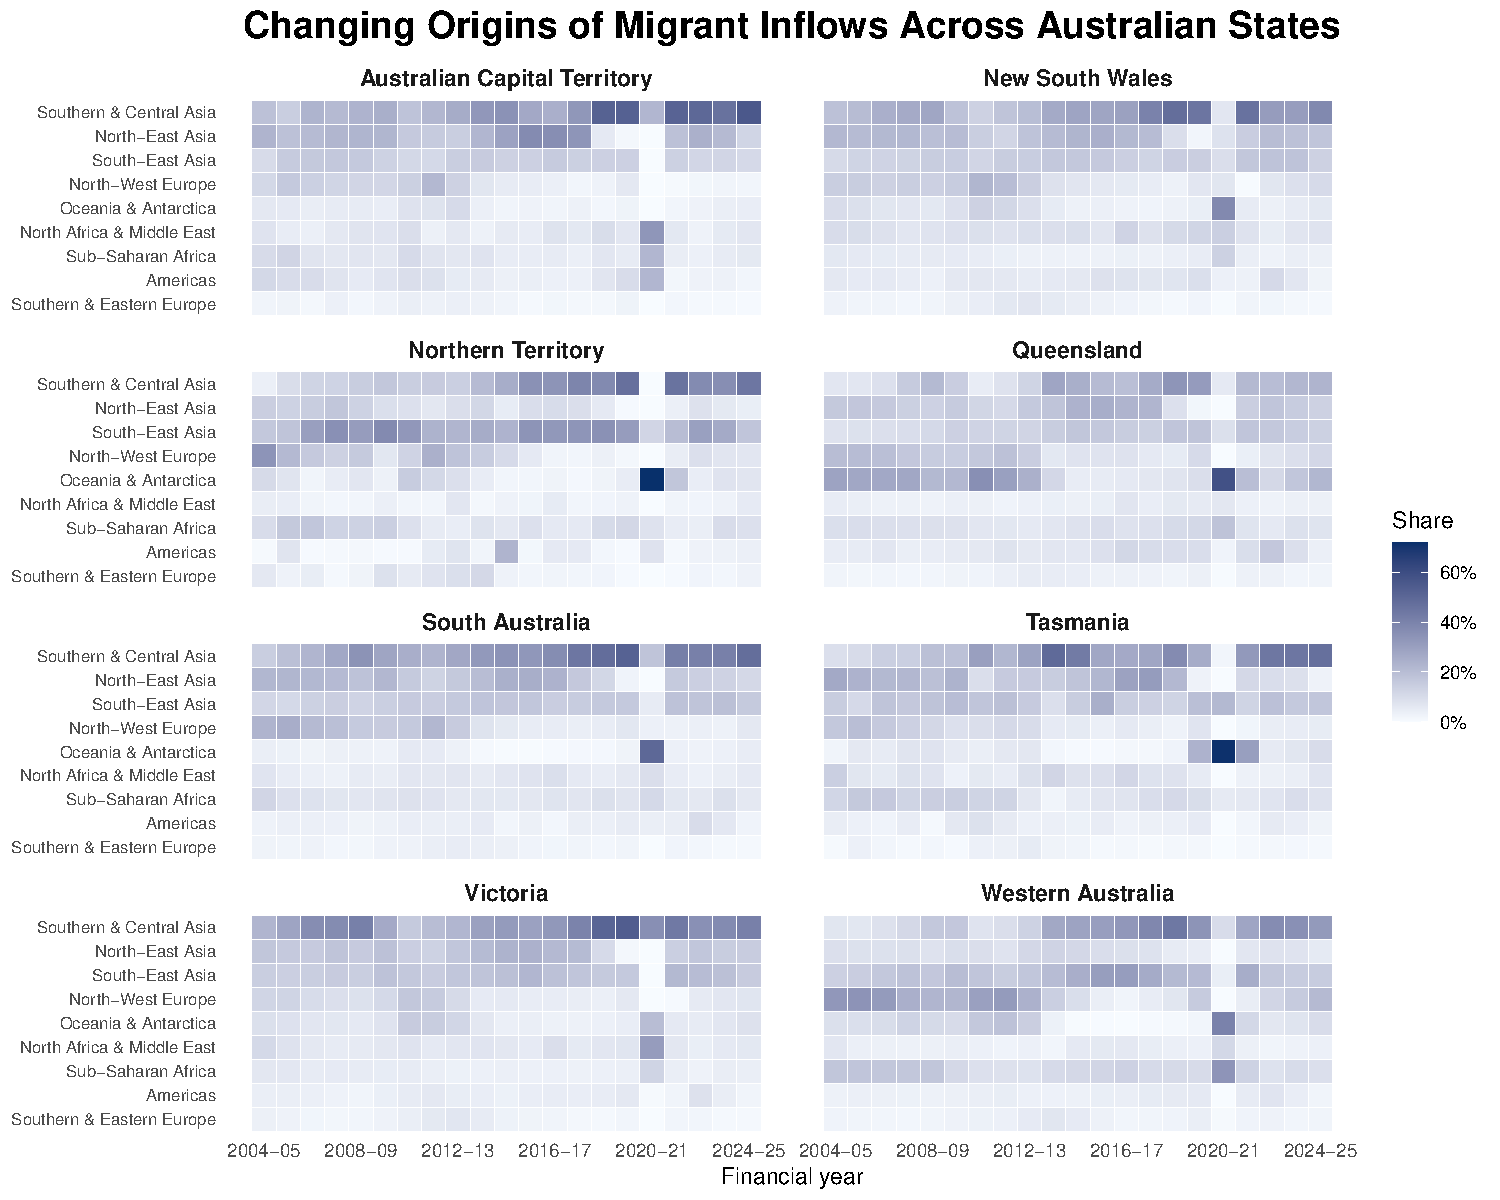
\includegraphics[keepaspectratio]{DEP_Wu_35717343_files/figure-pdf/fig-q2-origin-heatmap-1.pdf}}

}

\caption{\label{fig-q2-origin-heatmap}Origin composition of positive
overseas migrant inflows across Australian states, 2004-05 to 2024-25.
Darker tiles indicate larger shares within each state-year.}

\end{figure}%

\subsubsection{Within-state relationships between migrant-origin
concentration and economic
outcomes}\label{within-state-relationships-between-migrant-origin-concentration-and-economic-outcomes}

To summarise the relationship more clearly, I estimated a separate
within-state slope for each state rather than plotting all state-years
directly. Migrant-origin concentration was measured using a Herfindahl
index (HHI), where higher values indicate that migrant inflows were
concentrated in fewer countries of birth. I then examined whether years
with relatively higher concentration within each state also tended to
have relatively higher wage growth or housing lending growth. To reduce
the influence of unusual observations, I used robust regression and
plotted the resulting coefficients with 95\% confidence intervals in
Figure~\ref{fig-q2-within-state-coef}. Further calculation details for
this within-state analysis are provided in the
\hyperref[sec-appendix-within-state]{Appendix}.

In Figure~\ref{fig-q2-within-state-coef}, positive coefficients indicate
that, within a state, years with more concentrated migrant inflows
tended to coincide with stronger-than-usual economic growth, while
negative coefficients indicate the opposite. In the wage-growth panel, 7
of the 8 states have negative coefficients, with the strongest negative
slopes appearing in New South Wales (-29.5) and the Australian Capital
Territory (-23.5). The confidence intervals for New South Wales,
Victoria, Tasmania, and the Australian Capital Territory remain below
zero, suggesting that higher migrant-origin concentration was associated
with weaker-than-usual wage growth in these states.

By contrast, the housing-lending panel is more mixed, with 5 of the 8
states have positive coefficients, but only Northern Territory and
Tasmania have intervals that remain clearly above zero, with estimated
slopes of about 141.1 and 273.5 respectively. The remaining states have
wide intervals that cross zero. Overall, these results suggest that
while migrant origins and settlement patterns changed substantially
across states, higher migrant-origin concentration was more consistently
linked to weaker wage growth than to housing lending growth, and its
relationship with housing lending remained uneven across Australia.

\begin{figure}

\centering{

\pandocbounded{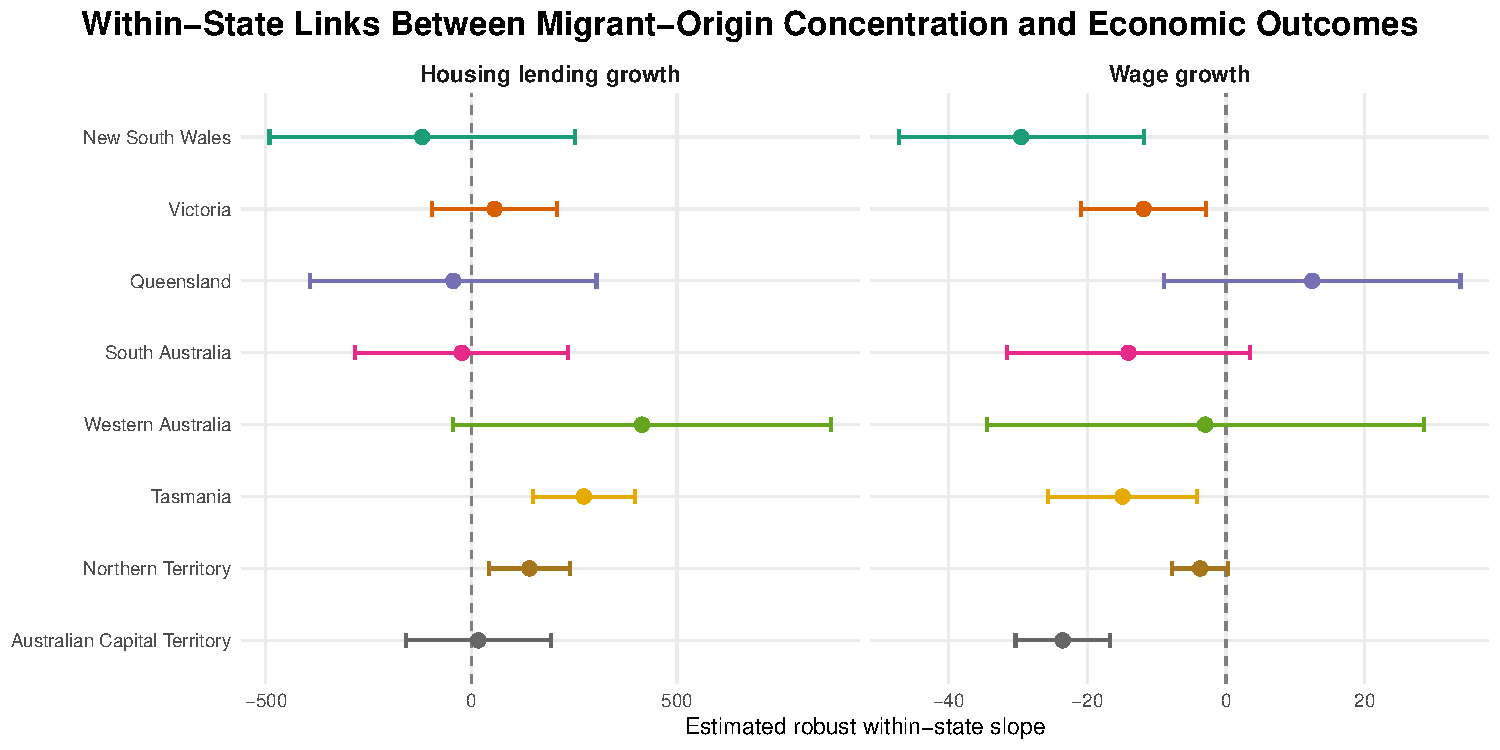
\includegraphics[keepaspectratio]{DEP_Wu_35717343_files/figure-pdf/fig-q2-within-state-coef-1.pdf}}

}

\caption{\label{fig-q2-within-state-coef}Robust within-state
associations between migrant-origin concentration and economic outcomes,
2005-06 to 2024-25. Coefficients are estimated from state-specific
robust regressions using deviations from each state's own average level.
Positive coefficients indicate that years with above-average
migrant-origin concentration tend to coincide with above-average
economic growth within the same state.}

\end{figure}%

\subsubsection{Summary of findings}\label{summary-of-findings-1}

Overall, Figure~\ref{fig-q2-origin-heatmap} and
Figure~\ref{fig-q2-within-state-coef} suggest that the origins of
overseas migrants and their settlement patterns changed substantially
across Australian states over time. Migrant inflows became increasingly
dominated by Southern and Central Asia, but this shift was not uniform
across Australia, with Victoria and the Australian Capital Territory
showing stronger concentration in Southern and Central Asian inflows,
while Western Australia retained a more visible North-West European
component. However, these changes in migrant origins were not associated
with stronger economic outcomes in any consistent way. Within states,
higher migrant-origin concentration was more often linked to weaker wage
growth, while its relationship with housing lending growth was mixed and
uneven across Australia.

\subsection{Where are the largest gaps between investor lending and
migration demand across Australian states, and how has this geography
changed over
time?}\label{where-are-the-largest-gaps-between-investor-lending-and-migration-demand-across-australian-states-and-how-has-this-geography-changed-over-time}

To reduce the influence of unusually disrupted migration patterns during
the pandemic period and the immediate reopening adjustment, I exclude
2020-21 to 2022-23 from the mapped comparison. I then compare three
representative periods, namely an earlier period (2004-05 to 2011-12), a
middle period (2012-13 to 2019-20), and a recent period (2023-24 to
2024-25). Averaging within each period makes state differences easier to
compare visually.

In Figure~\ref{fig-q3-maps}, blue states indicate that investor lending
is stronger than migration demand, while orange states indicate the
opposite. Queensland remains blue throughout, although the shade becomes
lighter in the middle period before returning to a stronger blue in the
recent period. Western Australia, by contrast, remains consistently
orange across all three maps. Northern Territory stays close to neutral
overall, but shifts slightly towards light orange in the middle and
recent periods. New South Wales shows the clearest positive shift,
moving from near-neutral in the earlier period to a much darker blue in
the middle period and then remaining strongly blue in the recent period.
Australian Capital Territory and Tasmania show a similar pattern,
staying close to neutral throughout, with only a small movement from
slightly blue towards slightly orange. South Australia is less stable,
shifting from slightly blue to orange in the middle period before
returning to near neutral in the recent period. Victoria shows the
clearest negative pattern, remaining orange in all three periods and
becoming darker over time.

Overall, Figure~\ref{fig-q3-maps} suggests that the investor--migration
gap becomes less even over time. The strongest mismatches are
concentrated in a small number of states, especially New South Wales and
Victoria, but in opposite directions. This pattern is consistent with
Figure~\ref{fig-q1-structure-value}, where New South Wales appears as
the most investor-oriented market, and it also complements
Figure~\ref{fig-q2-origin-heatmap}, which shows that migrant settlement
patterns remain uneven across states. Further calculation details for
this gap measure are provided in Section~\ref{sec-appendix-q3-gap}.

\begin{figure}

\centering{

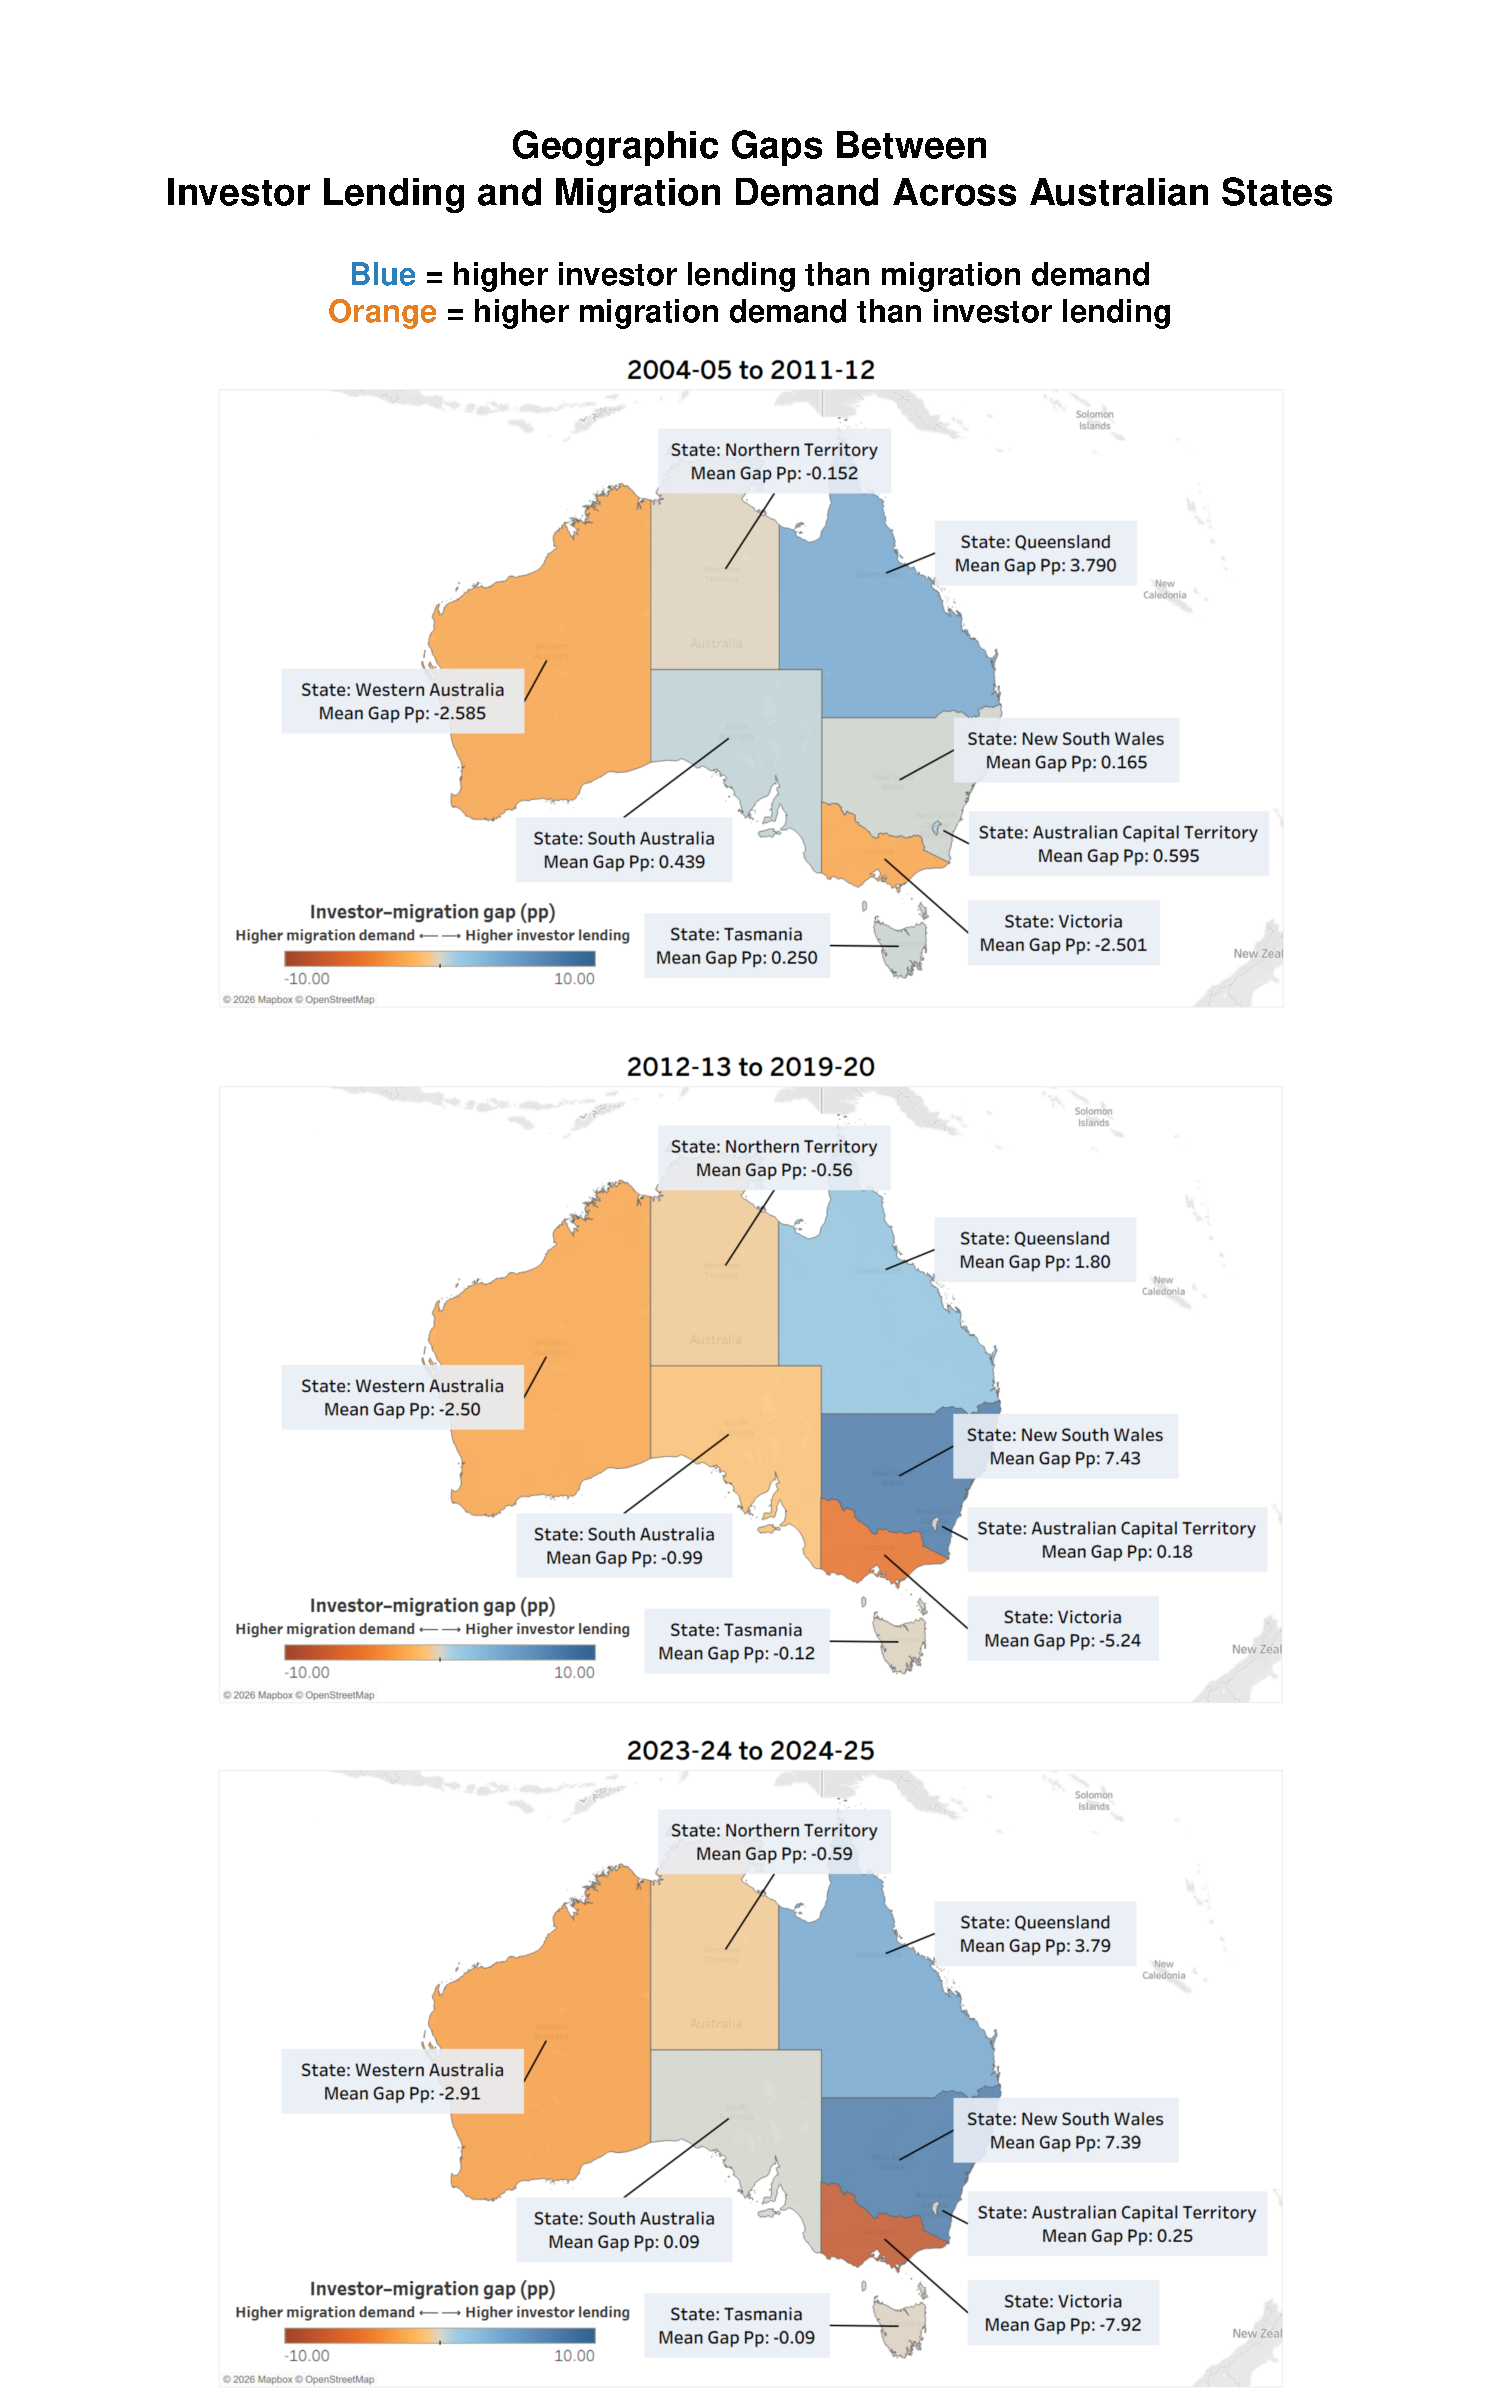
\includegraphics[width=1\linewidth,height=\textheight,keepaspectratio]{DEP_Wu_35717343_files/figure-pdf/fig-q3-maps-1.pdf}

}

\caption{\label{fig-q3-maps}Average gaps between investor lending share
and migration-demand share across Australian states in three
representative periods. Positive values indicate that a state's share of
investor lending exceeded its share of migration demand, while negative
values indicate the opposite.}

\end{figure}%

\clearpage

\section{Conclusion}\label{conclusion}

\section{Reflection}\label{reflection}

\section{References}\label{references}

\appendix

\section{Appendix}\label{appendix}

\subsection{Key calculated values for Housing Lending, Wage Growth and
Lending Structure Across Australian
States}\label{key-calculated-values-for-housing-lending-wage-growth-and-lending-structure-across-australian-states}

This appendix reports the main calculated values cited in Questions 1
and 2.

For Question 1, annual growth rates were calculated as:

\[
Growth_{st} = \left(\frac{X_{st}}{X_{s,t-1}} - 1\right)\times 100
\]

where \(X_{st}\) is the annual value for state \(s\) in financial year
\(t\).

The investor share of total housing lending value was calculated as:

\[
InvestorShare_{st} = \frac{InvestorValue_{st}}{InvestorValue_{st} + OwnerOccupierValue_{st}}
\]

The proportion of years in which a state's investor share exceeded the
national share was calculated as:

\[
AboveNational_s = \frac{1}{T}\sum_t I\left(Share_{st} > Share^{AUS}_t\right)
\]

where \(I(\cdot)\) is an indicator that takes the value 1 when the
condition is true and 0 otherwise.

\subsubsection{Main values cited in the annual growth
discussion}\label{main-values-cited-in-the-annual-growth-discussion}

\begin{longtable}[t]{lr}

\caption{\label{tbl-app-q1-growth-values}Main values cited in the
discussion of annual housing lending growth and wage growth}

\tabularnewline

\\
\toprule
Measure & Value\\
\midrule
National wage growth minimum & 1.5\%\\
National wage growth maximum & 4.2\%\\
National average wage growth & 3\%\\
\bottomrule

\end{longtable}

\subsubsection{Main values cited in the investor-share
discussion}\label{main-values-cited-in-the-investor-share-discussion}

\begin{longtable}[t]{>{\raggedright\arraybackslash}p{6cm}lcr}

\caption{\label{tbl-app-q1-investor-values}Main values cited in the
discussion of long-run changes in the investor share of lending value}

\tabularnewline

\\
\toprule
Measure & Geography & Financial year & Value\\
\midrule
National investor share at start of period & Australia & 2004-05 & 38.3\%\\
National investor share at peak & Australia & 2014-15 & 44.5\%\\
National investor share at trough & Australia & 2020-21 & 25.4\%\\
National investor share in latest year & Australia & 2024-25 & 37.8\%\\
New South Wales average investor share & New South Wales & 2004-05 to 2024-25 & 39.6\%\\
\addlinespace
New South Wales share above national benchmark & New South Wales & 2004-05 to 2024-25 & 81.0\%\\
New South Wales peak investor share & New South Wales & 2014-15 & 53.9\%\\
Tasmania average investor share & Tasmania & 2004-05 to 2024-25 & 25.8\%\\
Northern Territory investor share in latest year & Northern Territory & 2024-25 & 40.5\%\\
Tasmania investor share in latest year & Tasmania & 2024-25 & 26.2\%\\
\addlinespace
Western Australia investor share in 2020-21 & Western Australia & 2020-21 & 16.1\%\\
Western Australia investor share in latest year & Western Australia & 2024-25 & 36.8\%\\
\bottomrule

\end{longtable}

\subsection{Further calculation details for Within-State Links Between
Migrant-Origin Concentration and Economic
Outcomes}\label{further-calculation-details-for-within-state-links-between-migrant-origin-concentration-and-economic-outcomes}

This appendix provides further details of the calculation used in the
figure titled \emph{Within-State Links Between Migrant-Origin
Concentration and Economic Outcomes}.

For each state \(s\) and financial year \(t\), migrant-origin
concentration was measured using a country-level Herfindahl index (HHI):

\[
HHI_{st} = \sum_i p_{ist}^2
\]

where \(p_{ist}\) is the share of positive net overseas migration from
country of birth \(i\) in state \(s\) and year \(t\). It was calculated
as:

\[
p_{ist} = \frac{\max(\mathrm{NOM}_{ist}, 0)}{\sum_j \max(\mathrm{NOM}_{jst}, 0)}
\]

A higher HHI indicates that migrant inflows were more concentrated in
fewer countries of birth, while a lower HHI indicates a more diverse
origin mix.

To focus on within-state variation rather than long-run differences
between states, migrant-origin concentration, wage growth, and housing
lending growth were centred around each state's own average level:

\[
HHI^{dev}_{st} = HHI_{st} - \bar{HHI}_s
\]

\[
WAGE^{dev}_{st} = WAGE_{st} - \overline{WAGE}_s
\]

\[
LEND^{dev}_{st} = LEND_{st} - \overline{LEND}_s
\]

where \(\bar{HHI}_s\), \(\overline{WAGE}_s\), and \(\overline{LEND}_s\)
are the long-run state averages for each state.

Separate robust regression models were then estimated for each state.
For wage growth, the model was:

\[
WAGE^{dev}_{st} = \alpha_s + \beta_s HHI^{dev}_{st} + \varepsilon_{st}
\]

For housing lending growth, the model was:

\[
LEND^{dev}_{st} = \alpha_s + \beta_s HHI^{dev}_{st} + \varepsilon_{st}
\]

The coefficient \(\beta_s\) measures whether years with above-average
migrant-origin concentration within a state also tended to have
above-average wage growth or housing lending growth in that same state.
Robust regression was used so that unusual observations had less
influence on the estimated slopes than in ordinary least squares. The
intervals shown in the figure are approximate 95\% confidence intervals
based on the robust standard errors of the fitted models.

\subsubsection{Main values cited in the origin-composition
discussion}\label{main-values-cited-in-the-origin-composition-discussion}

\begin{longtable}[t]{>{\raggedright\arraybackslash}p{6cm}lcr}

\caption{\label{tbl-app-q2-origin-values}Main values cited in the
discussion of changing migrant origins across Australian states}

\tabularnewline

\\
\toprule
Measure & Geography & Financial year & Value\\
\midrule
Southern and Central Asia share of positive overseas migrant inflows & Australia & 2004-05 & 15.6\%\\
Southern and Central Asia share of positive overseas migrant inflows & Australia & 2024-25 & 36.3\%\\
Southern and Central Asia share of positive inflows & Australian Capital Territory & 2024-25 & 55.6\%\\
Southern and Central Asia share of positive inflows & Victoria & 2024-25 & 41.0\%\\
North-West Europe share of positive inflows & Western Australia & 2024-25 & 21.0\%\\
\bottomrule

\end{longtable}

\subsubsection{Main values cited in the robust within-state regression
discussion}\label{main-values-cited-in-the-robust-within-state-regression-discussion}

\begin{longtable}[t]{llrc}

\caption{\label{tbl-app-q2-robust-values}Main robust regression
coefficients and confidence intervals cited in the within-state analysis
of migrant-origin concentration and economic outcomes}

\tabularnewline

\\
\toprule
State & Economic outcome & Estimate & 95\% CI\\
\midrule
Australian Capital Territory & Wage growth & -23.5 & {}[-30.3, -16.7]\\
New South Wales & Wage growth & -29.5 & {}[-47.1, -11.9]\\
Tasmania & Wage growth & -14.9 & {}[-25.6, -4.2]\\
Victoria & Wage growth & -11.9 & {}[-20.9, -2.8]\\
Northern Territory & Housing lending growth & 141.1 & {}[41.9, 240.4]\\
\addlinespace
Tasmania & Housing lending growth & 273.5 & {}[149.7, 397.3]\\
\bottomrule

\end{longtable}

\subsection{Further calculation details for Geographic Gaps Between
Investor Lending and Migration Demand}\label{sec-appendix-q3-gap}

This appendix provides further details of the calculation used in the
figure titled \emph{Geographic Gaps Between Investor Lending and
Migration Demand Across Australian States}.

For each state \(s\) and financial year \(t\), migration demand was
proxied by the state share of positive overseas migrant inflows:

\[
MigrationShare_{st} = \frac{PositiveNOM_{st}}{\sum_r PositiveNOM_{rt}}
\]

where \(PositiveNOM_{st}\) is the total positive net overseas migration
in state \(s\) and year \(t\), aggregated across all countries of birth
except Australia. Positive inflows were used so that the measure
captured the distribution of incoming migration demand across states.

Investor activity was measured by the state share of investor lending
value:

\[
InvestorShare_{st} = \frac{InvestorValue_{st}}{\sum_r InvestorValue_{rt}}
\]

where \(InvestorValue_{st}\) is the total value of investor housing
lending in state \(s\) and year \(t\).

The investor--migration gap was then calculated as:

\[
Gap_{st} = 100 \times \left( InvestorShare_{st} - MigrationShare_{st} \right)
\]

This gap is expressed in percentage points. Positive values indicate
that a state's share of investor lending was larger than its share of
migration demand, while negative values indicate the opposite.

The mapped comparison excludes 2020-21 to 2022-23. These years were
heavily affected by COVID-19 border closures and the immediate
border-reopening adjustment, which produced unusually disrupted
migration patterns and made them less suitable for describing a stable
geographic relationship between investor lending and migration demand.

Instead, the mapped results were summarised over three representative
periods: - 2004-05 to 2011-12, - 2012-13 to 2019-20, - 2023-24 to
2024-25.

The first two periods divide the full pre-COVID sample into two
equal-length stages, which avoids dropping intermediate years without a
clear reason and makes the pre-COVID averages more comparable. The final
period captures the most recent post-disruption geography using the
latest available years.

For each state \(s\) and period \(p\), the mapped value was the average
of the annual gap over all years in that period:

\[
\overline{Gap}_{sp} = \frac{1}{T_p}\sum_{t \in p} Gap_{st}
\]

where \(T_p\) is the number of financial years in period \(p\).

The maps therefore summarise how strongly investor lending and migration
demand were aligned or misaligned across states in each of the three
selected periods.

\subsubsection{Largest positive and negative gaps in each
period}\label{largest-positive-and-negative-gaps-in-each-period}

\begin{longtable}[t]{lllr}

\caption{\label{tbl-app-q3-key-values}Largest positive and negative
investor--migration gaps across the three representative periods}

\tabularnewline

\\
\toprule
Period & Type & State & Gap (pp)\\
\midrule
2004-05 to 2011-12 & Largest positive gap & Queensland & 3.8\\
2012-13 to 2019-20 & Largest positive gap & New South Wales & 7.4\\
2023-24 to 2024-25 & Largest positive gap & New South Wales & 7.4\\
2004-05 to 2011-12 & Largest negative gap & Western Australia & -2.6\\
2012-13 to 2019-20 & Largest negative gap & Victoria & -5.2\\
\addlinespace
2023-24 to 2024-25 & Largest negative gap & Victoria & -7.9\\
\bottomrule

\end{longtable}

\subsubsection{Average investor--migration gaps by state and
period}\label{average-investormigration-gaps-by-state-and-period}

\begin{longtable}[t]{lrrrrr}

\caption{\label{tbl-app-q3-change-values}Average investor--migration
gaps by state and period, with changes over time}

\tabularnewline

\\
\toprule
State & 2004-05 to 2011-12 & 2012-13 to 2019-20 & 2023-24 to 2024-25 & Change: early to recent & Change: pre-COVID to recent\\
\midrule
New South Wales & 0.2 & 7.4 & 7.4 & 7.2 & 0.0\\
Queensland & 3.8 & 1.8 & 3.8 & 0.0 & 2.0\\
Western Australia & -2.6 & -2.5 & -2.9 & -0.3 & -0.4\\
Tasmania & 0.2 & -0.1 & -0.1 & -0.3 & 0.0\\
Australian Capital Territory & 0.6 & 0.2 & 0.2 & -0.3 & 0.1\\
\addlinespace
South Australia & 0.4 & -1.0 & 0.1 & -0.3 & 1.1\\
Northern Territory & -0.2 & -0.6 & -0.6 & -0.4 & 0.0\\
Victoria & -2.5 & -5.2 & -7.9 & -5.4 & -2.7\\
\bottomrule

\end{longtable}




\end{document}
